\documentclass[paper=letter, fontsize=11pt]{scrartcl}

\usepackage[T1]{fontenc}
\usepackage{fourier}
\usepackage[english]{babel}
\usepackage{amsmath,amsfonts,amsthm}
\usepackage{lipsum} % Used for inserting dummy 'Lorem ipsum' text into the template
\usepackage{sectsty} % Allows customizing section commands
\usepackage[latin1]{inputenc}

\usepackage{tikz}
\usetikzlibrary{shapes,arrows}
\tikzstyle{decision} = [diamond, draw, fill=green!20, 
    text width=4.5em, text badly centered, node distance=3cm, inner sep=0pt]
\tikzstyle{block} = [rectangle, draw, fill=blue!20, 
    text width=7em, text centered, rounded corners, minimum height=4em]
\tikzstyle{line} = [draw, -latex']
\tikzstyle{cloud} = [draw, ellipse,fill=red!20, node distance=3cm,
    minimum height=2em]

\allsectionsfont{\centering \normalfont\scshape} % Make all sections centered, the default font and small caps
\usepackage{fancyhdr}
\pagestyle{fancyplain}
\fancyhead[L]{\emph{Harvard University, CS165}}
\fancyhead[R]{Kevin Zhang}
\fancyfoot[L]{}
\fancyfoot[C]{\thepage}
\fancyfoot[R]{}
\renewcommand{\headrulewidth}{0pt}
\renewcommand{\footrulewidth}{0pt}
\setlength{\headheight}{8.6pt}
\numberwithin{equation}{section}
\numberwithin{figure}{section}
\numberwithin{table}{section}
\setlength\parindent{0pt}
\newcommand{\horrule}[1]{\rule{\linewidth}{#1}}
\usepackage{soul}
\definecolor{ivory}{rgb}{0.90, 0.90, 0.90}
\sethlcolor{ivory}
\renewcommand{\texttt}[1]{\hl{\ttfamily #1}}
\newcommand{\ttt}[1]{\hl{\ttfamily #1}}

\title{	
\normalfont \normalsize 
\horrule{0.5pt} \\[0.4cm]
\huge CS165 Final Report
}
\author{Kevin Zhang}
\date{\normalsize\today}
\begin{document}
\maketitle

\horrule{0.5pt}
\section{Feature Overview}
Almost all of the basic features requested of this project have been implemented.  The last features remaining at the moment are nested-loop joins and updates.  The list of features includes:
\begin{itemize}
	\item Creates - create a database, table, column, or index.
	\item Inserts - insert a row into any table.
	\item Selects - select data using a range operator on any column.
	\item Fetches - fetch data after selecting.
	\item Loads - load data from files into the database.
	\item Indexes - create indexes over columns for faster selects.
	\item Joins - join values across tables to construct additional tuples.
\end{itemize}
In addition, deletion in B+ trees has been implemented and tested to work (but not incorporated into updates yet).
\\\\Code has been organized according to project components; the Makefile used looks in several pre-defined folders for source and header files.  Header files mirror the layout of the source files.  In addition, a \texttt{data} folder stores all database metadata and values (persisted upon server shutdown and loaded upon server startup).  This folder (along with subfolders) is automatically created when needed.  A \texttt{catalog} file at the root contains database metadata.
\\\\Extensive logging has been implemented; when turned on, all queries, server responses, client messages, and more are printed to stdout.  In addition, after execution of each query and on startup, the current database and client context are printed to help debug.

\horrule{0.5pt} 
\section{System Overview}
The diagram below details how queries are handled by the server.
    
\begin{center}
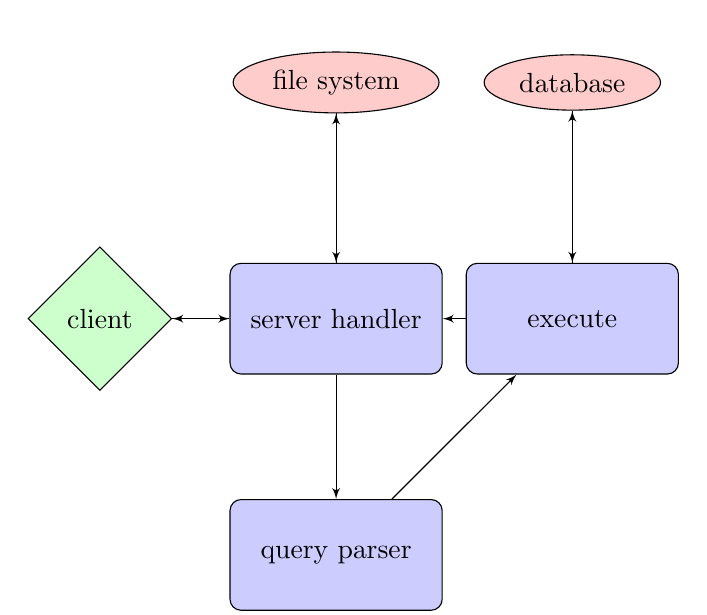
\begin{tikzpicture}[node distance = 2cm, auto]
    % Place nodes
    \node [decision] (init) { client };
    \node [block, right of=init, node distance=3cm] (server) { server handler };
    \node [block, below of=server, node distance=3cm] (parse) { query parser };
    \node [block, right of=server, node distance=3cm] (execute) { execute };
    \node [cloud, above of=execute, node distance=3cm] (db) { database };
    \node [cloud, above of=server, node distance=3cm] (system) { file system };
    \path [line] (init) -- (server);
    \path [line] (server) -- (init);
    \path [line] (server) -- (parse);
    \path [line] (parse) -- (execute);
    \path [line] (execute) -- (db);
    \path [line] (db) -- (execute);
    \path [line] (execute) -- (server);
    \path [line] (server) -- (system);
    \path [line] (system) -- (server);
\end{tikzpicture}
\end{center}

Green nodes indicate sections the user interacts with, red nodes indicate data sources, and purple nodes indicate server functions.  On a client request, the following actions are taken:
\begin{enumerate}
	\item Request is forwarded from server handler to query parser.
	\item Query parser constructs a \texttt{DbOperator} object and passes it to the executor.
	\item Executor interacts with the database to build a \texttt{Result} object if necessary.
	\item Executor returns a string response to the server.
	\item Server responds to the client if appropriate.
\end{enumerate}

The \texttt{DbOperator} object contains all metadata required to execute queries; a \texttt{ClientContext} object is used to store all \texttt{Result} objects created from queries.

\horrule{0.5pt} 
\section{Creates}
Handling create queries is fairly straightforward; on request, corresponding objects are created.  For a database, this is a \texttt{Db} object; for a table, a \texttt{Table} object; for a column, a \texttt{Column} object; and for an index, an \texttt{Index} object.  The \texttt{Db, Table, Column} objects contain straightforward fields describing the contents of each, along with pointers to payloads and contained objects.  
\\\\\texttt{Index} objects are a bit more complicated; these contain a \texttt{IndexType} identifying the \texttt{Index} as a B+ tree or column and a \texttt{clustered} descriptor.  \ttt{Index} objects additionally contain pointers to their respective \ttt{Column} objects (for ease of data lookup) and a \ttt{IndexObject}, which is either a \ttt{BTreeUNode} (unclustered B+ tree), \ttt{BTreeCNode} (clustered B+ tree), \ttt{ColumnIndex} (containing integer arrays of values and indices), or \ttt{NULL}, signifying a clustered, sorted index (no additional data is needed to maintain this type of index).
\\\\\ttt{Index} objects are stored in the corresponding \ttt{Table}.  Upon creation of a clustered index, no data is stored (it is assumed that clustered indices will be declared before any data is inserted into the database).  However, upon creation of unclustered indexes, all data is inserted into the indexes.  Thus, queries can immediately make use of the indexes (after insertion completes, of course).

\begin{center}
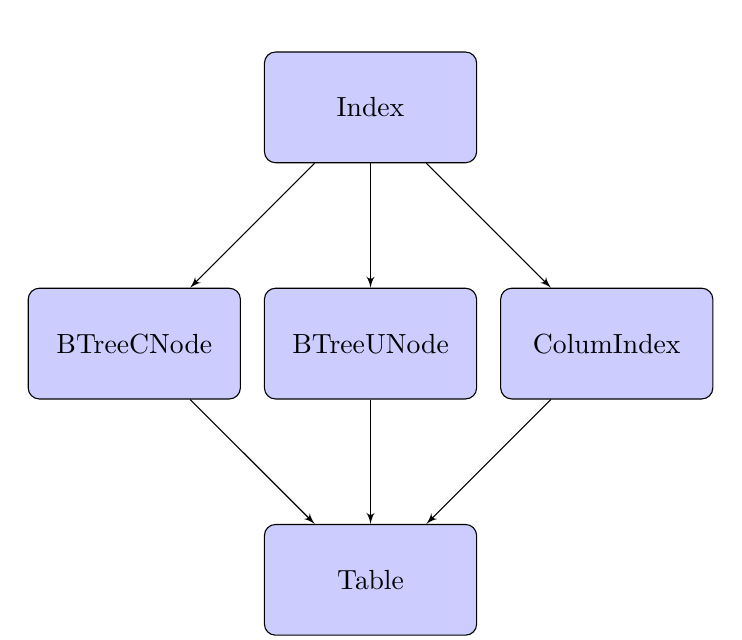
\begin{tikzpicture}[node distance = 2cm, auto]
\node [block] (index) { Index };
\node [block, below of=index, node distance = 3cm] (btreeu) { BTreeUNode };
\node [block, left of=btreeu, node distance = 3cm] (btreec) { BTreeCNode };
\node [block, right of=btreeu, node distance = 3cm] (cindex) { ColumIndex };
\node [block, below of=btreeu, node distance = 3cm] (table) { Table };
\path [line] (index) -- (btreec);
\path [line] (index) -- (btreeu);
\path [line] (index) -- (cindex);
\path [line] (btreec) -- (table);
\path [line] (btreeu) -- (table);
\path [line] (cindex) -- (table);
\end{tikzpicture}
\end{center}

\horrule{0.5pt} 
\section{Inserts}
Inserts without indexes are easy; we append to the end of the corresponding \ttt{Column} objects in the given \ttt{Table}.  Handling \ttt{Index} objects is harder.
\\\\The system completes the following process whenever inserting data:
\begin{enumerate}
\item Search for clustered indexes on the table.
\item If one is found, insert into the clustered index first (no more than one clustered index may exist).  Retrieve the indices of the inserted values, then shift all values in each column one by one (to avoid unnecessary random access) as necessary to insert new data.
\item If none are found, append all values to the end of the table, then insert the new \ttt{(value, index)} pairs into each of the unclustered indices.
\end{enumerate}

The B+ tree implementation is critical for this portion of the project (and probably the most time-consuming).  The optimal parameters for B+ trees have yet to be determined.

\begin{center}
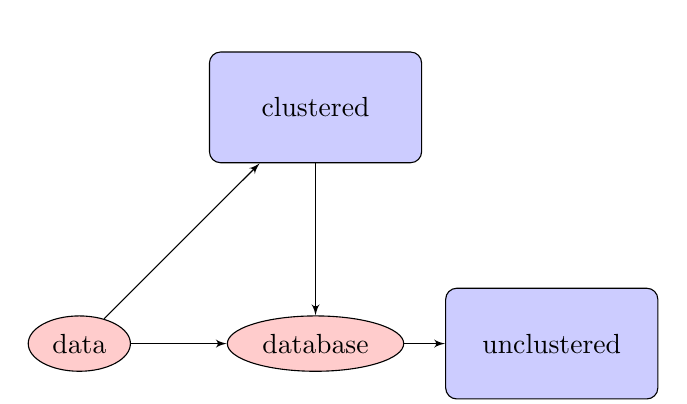
\begin{tikzpicture}[node distance = 3cm, auto]
\node [cloud] (db) { database };
\node [block, above of=db] (cluster) { clustered };
\node [block, right of=db] (uncluster) { unclustered };
\node [cloud, left of=db] (data) { data };
\path [line] (data) -- (db);
\path [line] (data) -- (cluster);
\path [line] (cluster) -- (db);
\path [line] (db) -- (uncluster);
\end{tikzpicture}
\end{center}

\horrule{0.5pt}
\section{Selects}
Selects without indexes are also easy; we simply scan through the entire column and append to a results array contained in the corresponding \ttt{ClientContext} object.  When we have a usable \ttt{Index}, we search through the \ttt{Index} to find the smallest value greater than or equal to the minimum of a select query.  Depending on the type of index, we then:
\begin{itemize}
\item Clustered B+ Tree: search for the maximum, then create an array containing all values between the two indexes found.
\item Clustered Sorted: binary search for the maximum, then create an array containing all values between the two indexes found.
\item Unclustered B+ Tree: iterate forward through the leaves until we find a value greater than the maximum, and accumulate an array of encountered indices.
\item Unclustered Sorted: iterate forward through the array until we find a value greater than the maximum, and accumulate an array of encountered indices.
\end{itemize}

For batched selects, this behavior is slightly modified:
\begin{itemize}
\item Clustered indexes: iterate across select queries first, building result arrays one by one.
\item Unclustered indexes: iterate down the index and build result arrays along the way.
\end{itemize}
For clustered indexes, we avoid leapfrogging between result arrays and instead write all values to each result array first.  This avoids some degree of random access.  For unclustered indexes, we avoid scanning the same data more than once and instead accumulate values as we go, avoiding multiple data scans but incurring costs from leapfrogging across result arrays instead.
\\\\Normal queries took the following amounts of time (50000 tuples, run in background):
\begin{table}[h!]
\centering
\begin{tabular}{c | c}
Select \% & \# us \\
9.1\% & 347 \\
18.2 \% & 384 \\
27.3 \% & 355 \\
36.4 \% & 388 \\
45.5 \% & 543 \\
54.6 \% & 518 \\
63.7 \% & 563 \\
72.8 \% & 540 \\
81.9 \% & 708 \\
90.9 \% & 635 \\
100 \% & 634
\end{tabular}
\end{table}

In total, these queries run independently would take 5615 microseconds.  Batched queries were able to consistently complete these queries in under 5000 microseconds; we would likely see a larger margin of improvement with a very large number of queries.  The largest number of concurrent queries we can run depends on how much space we have available for results.

\horrule{0.5pt}
\section{Fetches}
All fetches are done in the same way in this project; we iterate across the array of indices from a select query, and retrieve the corresponding values from the column in question.  The constructed \ttt{Index} objects are not as useful here, since keys into the indexes are values instead of indices.  An alternative implementation might maintain two sets of \ttt{Index} objects such that retrieving values using an indice is possible as well.  This incurs additional overhead, and does not solve the problem of random access.

\horrule{0.5pt}
\section{Loads}
Loads are done simply by sending row after row to the server.  An alternative implementation would batch all data, and utilize all data at once to construct the indexes.  This would decrease \ttt{Index} construction by a constant factor, since construction of each node is still required (this method also requires fairly expensive computation).

\horrule{0.5pt}
\section{Indexes}
Selects, inserts and fetches have been described for indexes above.  Sorted column indexes are straightforward.  There was not enough time to perform experiments to determine the optimal fan out, but, based off calculations on the page size (assuming 64K) and struct size, the optimal number of values stored in each node is around 2700.
\\\\We also recorded data on scan vs. index select performance.  Some of the results are shown below:

\begin{table}[h!]
\centering
\begin{tabular}{c | c | c}
Select \% & Scans & Indexes \\
0 \% & 220 & 1 \\
9.1 \% & 226 & 94 \\
18.2 \% & 197 & 71 \\
27.3 \% & 220 & 120 \\
36.4 \% & 349 & 188 \\
45.5 \% & 411 & 198 \\
54.6 \% & 530 & 238 \\
63.7 \% & 629 & 277 \\
72.8 \% & 704 & 347 \\
81.9 \% & 303 & 371 \\
90.0 \% & 325 & 415 \\
100.0 \% & 304 & 425
\end{tabular}
\caption{Runtime in milliseconds, 50000 tuples}
\end{table}


There is a clearly linear trend upwards for the indexes, while runtime seems to be mostly linear for scans up until around 80\% selectivity, when runtime drops again.  This is expected; runtime for indexes are dependent entirely on the number of values that need to be saved.  Scans are a bit more complex; deciding whether a value needs to be saved or not requires a branch, which can result in very slow behavior when values are randomly distributed and are close to 50\% selectivity.  This is what we see in our data; runtime increases up but then drops when branching behavior becomes more consistent.
\\\\Overall, indexes seem to perform better for lower selectivities, as expected.

\horrule{0.5pt}
\section{Joins}
Only hash joins have been implemented for now (nested joins are fairly trivial to implement).  These are implemented as follows: 
\begin{enumerate}
\item Insert all values from one select / fetch pair into a hashtable.
\item Iterate over all values from the other select / fetch pair.  For each value and index:
	\begin{itemize}
	\item Retrieve all indices from the hashtable with a matching value.
	\item Insert all indices into the first result handle.
	\item Insert as many copies of the index into the second result handle.
	\end{itemize}
\end{enumerate}

Again, there was not enough time to compare hash join performance with that of nested loops, but it seems reasonable to assume that, for low selectivities, hash joins are much more efficient than nested loop joins.  Experiments would be required to determine an exact boundary as a function of the \% selectivity and number of tuples.

\end{document}